Measurements of vector boson scattering (VBS) processes probe the non-Abelian gauge structure of the electroweak (EW) interactions of the standard model (SM) of particle physics. The discovery of a Higgs boson~\cite{Aad:2012tfa,Chatrchyan:2012xdj,CMSPaperCombinationLong} established that $\PW$ and $\PZ$ gauge bosons acquire mass via the Higgs mechanism. Models of physics beyond the SM predict enhancement in VBS processes through modifications of the Higgs boson couplings to gauge bosons~\cite{PhysRevD.87.055017, PhysRevD.87.093005}. 

At the LHC, VBS is characterized by presence of two gauge bosons in association with two forward jets with large rapidity separation and a large dijet mass. The VBS topology is produced via the EW interaction with increased sensitivity to quartic gauge couplings. Figure~\ref{fig:feynman} shows the Feynman diagrams involving quartic vertices. An excess of events with respect to SM predictions could indicate the presence of anomalous quartic gauge couplings (AQGCs)~\cite{aqgc_operators} or the existance of new resonances. 


\begin{figure*}[htb]
\centering
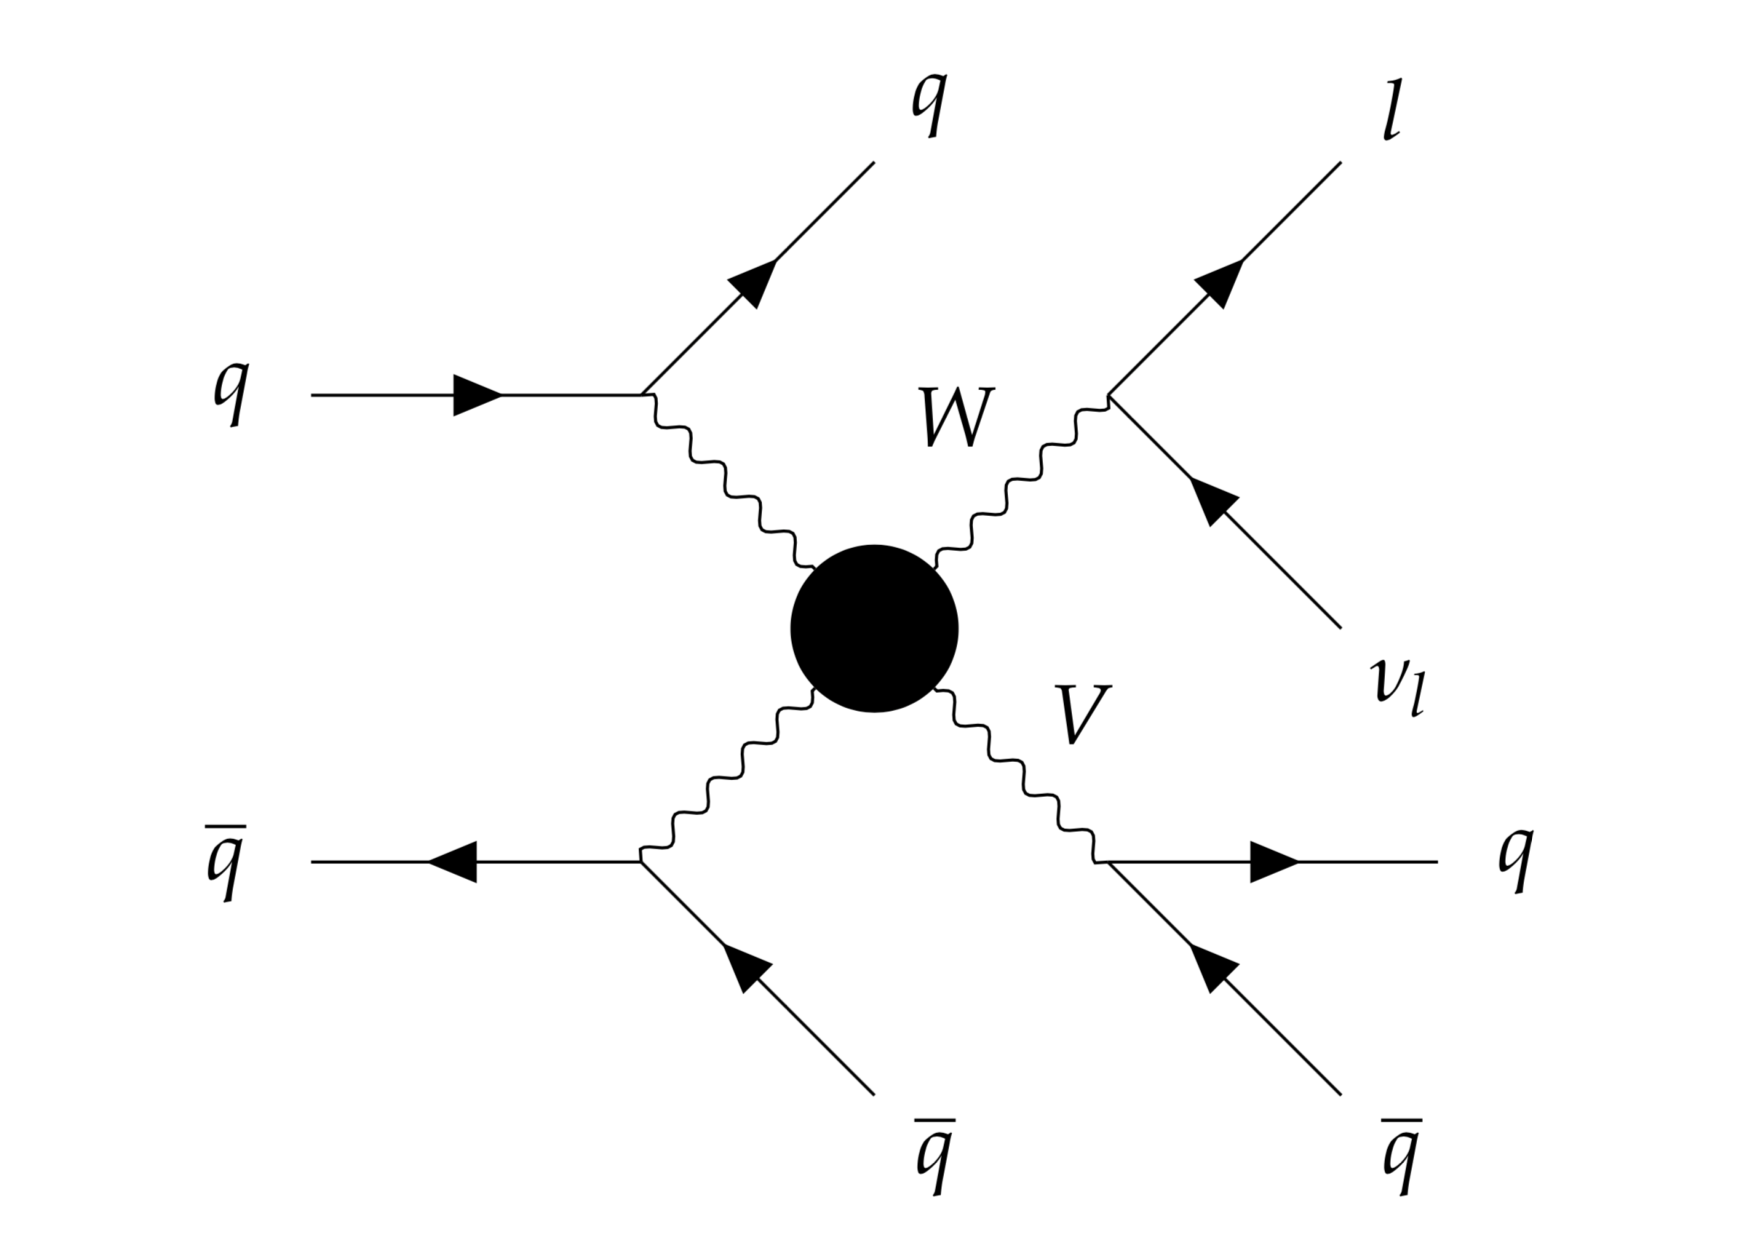
\includegraphics[width=\cmsFigWidth]{Plots/plots/FeynmanDiagram_WV.pdf}
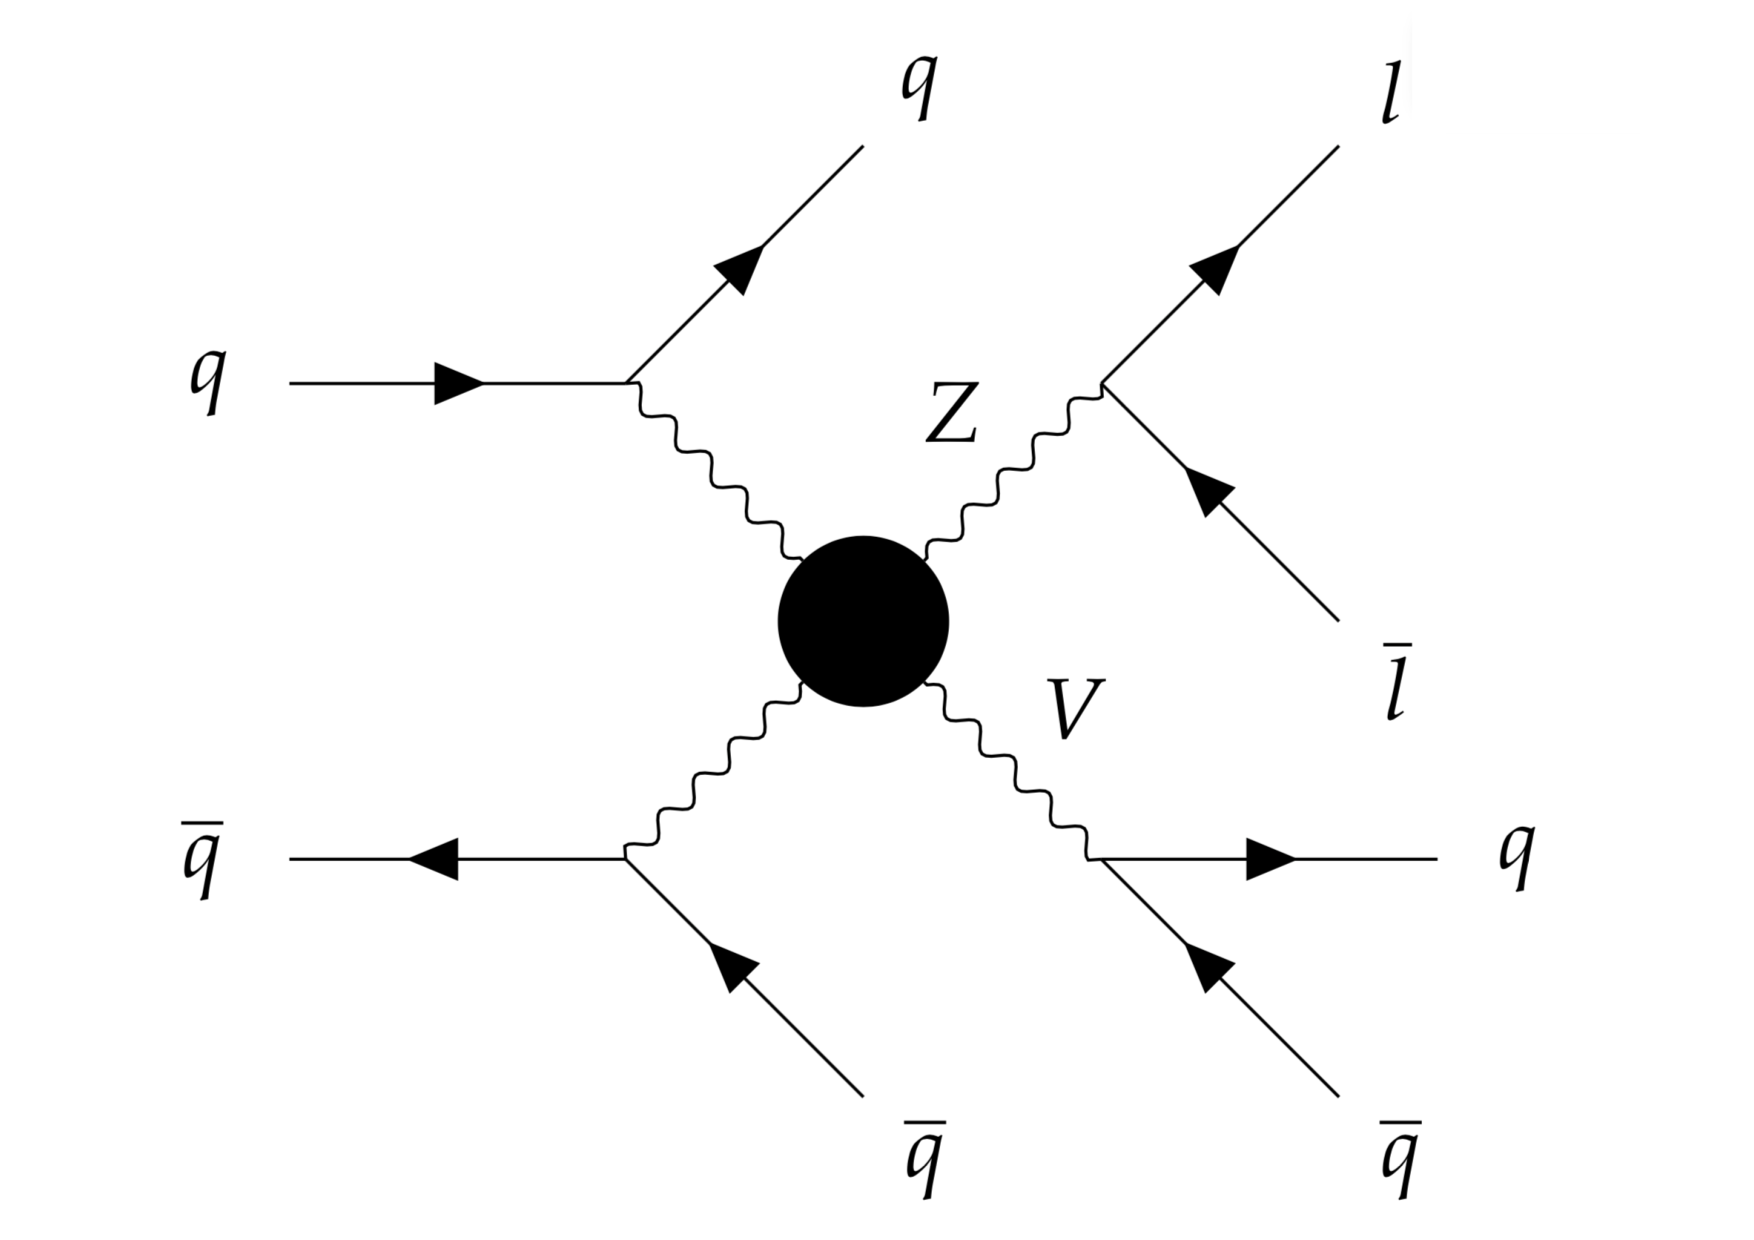
\includegraphics[width=\cmsFigWidth]{Plots/plots/FeynmanDiagram_ZV.pdf}
\caption{VBS Feynman diagrams contributing to the EW induced production of events containing a hadronically decaying gauge boson ($V$), a $\PW$ (left) or $\PZ$ (right) boson decaying to leptons (electrons or muons), and two forward jets. New physics in the EW sector can modify the quartic gauge coupling.}
\label{fig:feynman}
\end{figure*}


The main goal of this analysis is to search for the presence of AQGCs in candidate events containing a hadronically decaying gauge boson ($V$) produced with large transverse momentum $\pt$, a $\PW$ or $\PZ$ boson decaying to leptons (electrons or muons), and two forward jets. This final state benefits from a higher branching ratio of the $V$ decay compared to previous searches at the LHC for AQGCs in VBS involving only leptonic boson decays~\cite{Sirunyan:2017ret, ATLAS_ssWW, CMS_ssWW, Aaboud:2016ffv,Aad:2016ett, Sirunyan:2017fvv, Khachatryan:2016mud, Khachatryan:2017jub, Khachatryan:2016vif,Aaboud:2017pds}. The ATLAS collaboration reported limits on AQGCs in VBS using the $\PW V$ final state, where $\PW$ decays to leptons, in proton-proton (pp) collisions at $\sqrt{s}=8\TeV$. 

Extended Higgs sectors with additional SU(2) isotriplet scalar give rise to charged Higgs bosons with couplings to $\PW$ and $\PZ$ bosons at the tree level~\cite{CE1,CE2}. In particular, the Georgi-Machacek (GM)~\cite{GEORGI1985463} model, with both real and complex triplets,  preserves the tree level custodial symmetry. In this model, singly and doubly charged Higgs bosons are produced via vector boson fusion (VBF) and decay to $\PW$ and $\PZ$ bosons, and same-sign $\PW$ boson pairs, respectively. The ATLAS and CMS Collaborations performed searches for charged Higgs bosons in these topologies and set constraints on the GM model~\cite{Sirunyan:2017ret,Sirunyan:2017sbn,PhysRevLett.114.231801}.

This note presents a study of VBS in $\PW\PW$, $\PW\PZ$, and $\PZ\PZ$ final states using pp collisions at $\sqrt{s}=13\TeV$. The data sample corresponds to an integrated luminosity of $35.9 \pm 0.9\fbinv$ collected with the CMS detector~\cite{Chatrchyan:2008zzk} at the CERN LHC in 2016. 

